%\documentclass[main.tex]{subfiles}
%Edit
\lhead{Date taken: 9/25}
\chead{}
\rhead{Week One}
\author{Alice Michael}
\title{CS494 Notes}
\date{}
\begin{document}

%\noindent\large{\bf \textit{Challenges}}\\

%\begin{figure}[h!]
%\centering
%\includegraphics[width=0.8\linewidth]{addressSpace.jpg}
%\caption[Address Space]{Address Space}
%\label{fig:Address Space}
%\end{figure}	

%\begin{enumerate}
%  \itemsep-1.5em
%  \item 
%\end{enumerate}



%Edit
\section*{Packet Switching vs Circuit switching}
\noindent \large{\bf{The fundamental question in networking;\\
\indent\indent \textit{How is data transferred through the net?}}}\\
 \\
 \\
\noindent\large{\bf \textit{circuit switching:}}
\begin{itemize}
  \itemsep-1.5em
  \item End to end transfer\\
  \item all resources used\\
  \item Dedicated allocation\\
  \item reserved resources\\
\end{itemize}


\noindent\large{\bf \textit{packet switching:}}
\begin{itemize}
  \itemsep-1.5em
  \item chunks sent over the line at a time\\
  \item resources used in chunks\\
  \item If the number of packets arriving exceeds the number that can be serviced, they are dropped\\
  \item on-demand allocation\\
\end{itemize}
 \\

\noindent Great for: bursty data \arr resource sharing, simpler, no call setup\\
\noindent Bad for: Applications with hard resource requirements\\
    \indent Excessive congestion: packet delay and loss\\
    \indent Need protocols for reliable data transfer, and congestion control\\

\noindent How can we provide circuit-like behavior?\\
    \indent Bandwidth guarantees needed for audio/video apps\\
    \indent Common solution: over-povision\\

 \\
\newpage
\section*{Packet Switching: Statistical Multiplexing}
We can use statistics to pick the best option for scheduling of packets.  This will lower the amount of time that is wasted while elevating the speed things are transmitted\\
{\bf{Packet Switching allows more users to use the network by exploiting the randomness of the users.}}\\
\begin{figure}[h!]
\centering
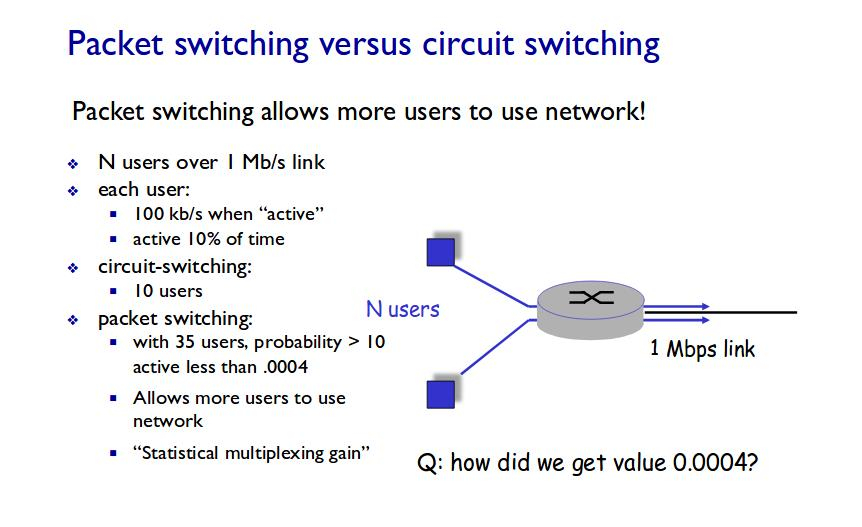
\includegraphics[width=0.8\linewidth]{Slide-A.jpg}
\caption[all the math]{all the math}
\label{fig:all the math}
\end{figure}	


\noindent $1$ Mbps / Each user needs $100$ kbps = $10^6$ bps / $100 x10^3$ bps\\
Probability that a user is active: 10\%\\


\newpage
\section*{4 Types of delay}

\noindent\large{\bf \textit{processing}} \arr determine output link, check bit errors\\

\noindent\large{\bf \textit{queueing}} \arr biggest portion of delay, it is the slowest\\
\indent\indent\indent\indent\arr time waiting at output link for transmission\\

\noindent\large{\bf \textit{transmission}}\\
R\arr link bandwidth in bits per second\\
L\arr packet length in bits\\
$D_t = L/R$ \\
 \\

\noindent\large{\bf \textit{propagation}}\\
d = length of physical link\\
s = propagation speed in medium\\
$D_{prop} = d/s$\\

\indent\indent\indent\indent\indent EX; Propagation Delay:\\
\indent\indent\indent\indent\indent Packet of length 1024 bytes\\
\indent\indent\indent\indent\indent        \arr $1024 * 8$ bits\\
\indent\indent\indent\indent\indent        \arr $8192$ bits\\

\indent\indent\indent\indent\indent Over 27 kbps dial up modem access limit\\
\indent\indent\indent\indent\indent        \arr $\frac{8192}{27*10^3}$ sec  \\
\indent\indent\indent\indent\indent        \arr 0.303 sec\\
\indent\indent\indent\indent\indent Over 10 Gbps Ethernet\\
\indent\indent\indent\indent\indent        \arr $\frac{8192 ~bits}{10*10^9 ~bits/sec}$ \\
\indent\indent\indent\indent\indent        \arr $8192$ nano sec\\
\indent\indent\indent\indent\indent        \arr $8192 * 10^{-7}$\\


\noindent Nodal Delay = $D_N = D_p + D_q + D_t + D_{prop}$
 \\
 \\
\noindent EX; Queueing Delay:\\
traffic intensity = $\frac{La}{R}$\\
